% !TeX program = xelatex
\documentclass[11pt]{article}
\usepackage[margin=0.8in]{geometry}
\usepackage{fontspec}
\setmainfont{Times New Roman}
\setsansfont{Arial}
\usepackage{graphicx,caption,hyperref,xurl}
\hypersetup{hidelinks,pdftitle={Computational Supplement},pdfsubject={Which Conclusions Does an Explanation Support? Claim-Scoped Diagnostic Gates for Interpretable Machine Learning in Psychology}}
\captionsetup{font=small,labelfont=bf,textfont=it,labelsep=newline,justification=raggedright,singlelinecheck=false}
\renewcommand{\thefigure}{CS\arabic{figure}}
\setlength{\parindent}{0pt}
\setlength{\emergencystretch}{2em}
\begin{document}
\special{pdf:trailerid [<520aa4199f8039b401bb3b1ba5b7c8bc> <520aa4199f8039b401bb3b1ba5b7c8bc>]}
\section*{Computational Supplement}
\textbf{Which Conclusions Does an Explanation Support? Claim-Scoped Diagnostic Gates for Interpretable Machine Learning in Psychology}\par
Stefan Coors, Clara S. Vetter, Jonas Hauck, Bernd Bischl, and Sven Hilbert\par
\medskip
This supplement shows the diagnostic displays of the applications to the Survey of Health, Impairment and Living Conditions in Denmark (SHILD) and the Programme for International Student Assessment (PISA) that Supplement F of the online supplement lists: calibration, subgroup comparisons, accumulated local effects (ALE), individual conditional expectation (ICE) curves, interaction surfaces, and differences in individual predictions across similarly accurate learners. No claim of the article depends on them. The figures are numbered CS1 to CS28 to distinguish them from the figures of the online supplement (S1 to S4).\par
\medskip
The SHILD displays describe the unweighted analytic sample of respondents who reported being satisfied or dissatisfied with their lives. The PISA displays describe the first plausible value of reading proficiency in the unweighted sample of 48,000 students from 32 countries, without design weights. None of the displays establishes causal effects, transport to other settings, or adequacy for decisions about individuals.\par
\medskip
Some labels inside the figures word things differently from the article: ``discontent'' denotes dissatisfaction with life, ``OOF'' (out of fold) denotes held-out predictions, ``PV1'' the first plausible value, ``p50'' the median, and ``ROC AUC'' the AUC.\par
\medskip
Abbreviations: ALE = accumulated local effects; AUC = area under the receiver operating characteristic curve; ICE = individual conditional expectation; PISA = Programme for International Student Assessment; RMSE = root mean squared error; SHILD = Survey of Health, Impairment and Living Conditions in Denmark; WLE = weighted likelihood estimate.\par
\medskip
The figure components and their aggregate source tables are in the analysis repository (\url{https://github.com/coorsaa/csdg-analysis}).
\clearpage
\begin{figure}[p]
\caption{SHILD flexible held-out calibration}
\label{supp:shild_g3_calibration}
\centering
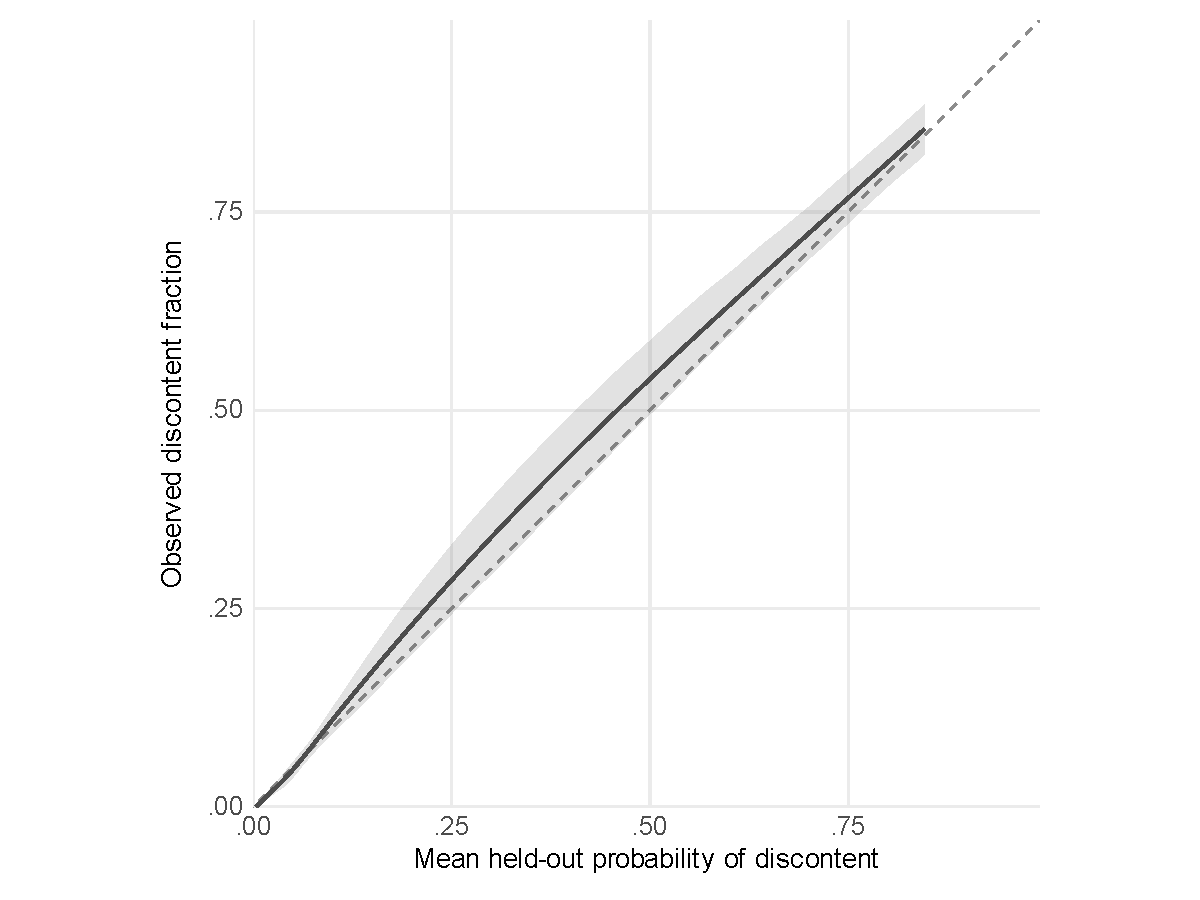
\includegraphics[width=.98\linewidth,height=5.6in,keepaspectratio]{shild/figures/shild_g3_calibration.pdf}
\par\smallskip{\raggedright\small\textit{Note.} The curve is a loess estimate; the band is a pointwise 95\% respondent-bootstrap percentile interval conditional on the supplied held-out predictions. It is neither simultaneous nor inclusive of model-training variation; the diagonal denotes perfect calibration.\par}
\end{figure}
\clearpage
\begin{figure}[p]
\caption{SHILD XGBoost subgroup AUC comparison, by age group}
\label{supp:shild_g7_subgroups__audit_age_group}
\centering
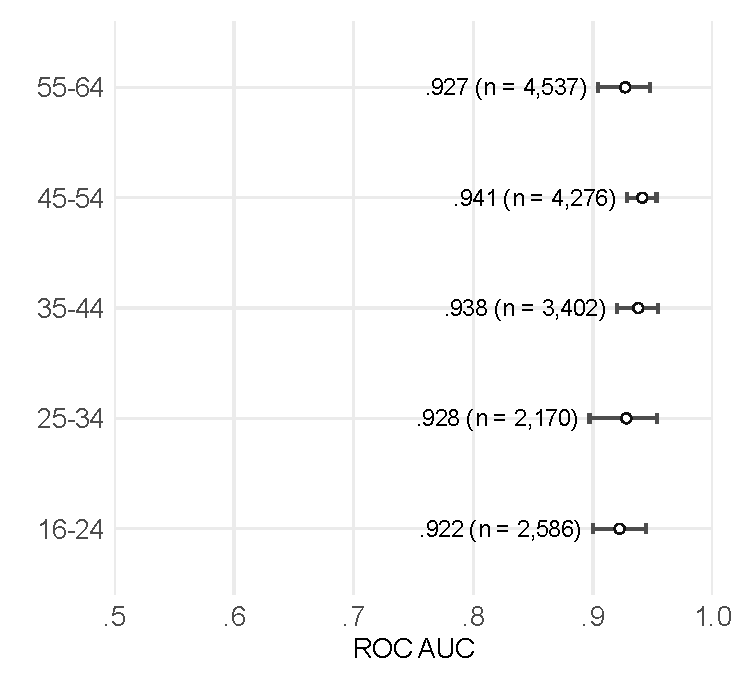
\includegraphics[width=.98\linewidth,height=5.6in,keepaspectratio]{shild/figures/shild_g7_subgroups__audit_age_group.pdf}
\par\smallskip{\raggedright\small\textit{Note.} Row-bootstrap 95\% intervals conditional on held-out predictions; direct labels show AUC and n.  The full .5–1.0 AUC scale avoids magnifying small absolute gaps.\par}
\end{figure}
\clearpage
\begin{figure}[p]
\caption{SHILD XGBoost subgroup AUC comparison, by gender}
\label{supp:shild_g7_subgroups__audit_gender}
\centering
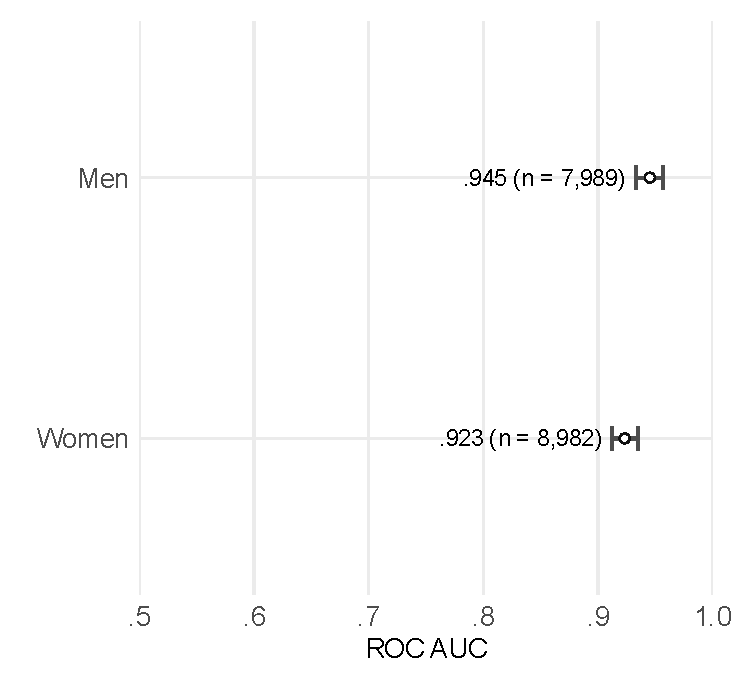
\includegraphics[width=.98\linewidth,height=5.6in,keepaspectratio]{shild/figures/shild_g7_subgroups__audit_gender.pdf}
\par\smallskip{\raggedright\small\textit{Note.} Row-bootstrap 95\% intervals conditional on held-out predictions; direct labels show AUC and n.  The full .5–1.0 AUC scale avoids magnifying small absolute gaps.\par}
\end{figure}
\clearpage
\begin{figure}[p]
\caption{SHILD pairwise subgroup AUC contrasts}
\label{supp:shild_g7_subgroup_contrasts}
\centering
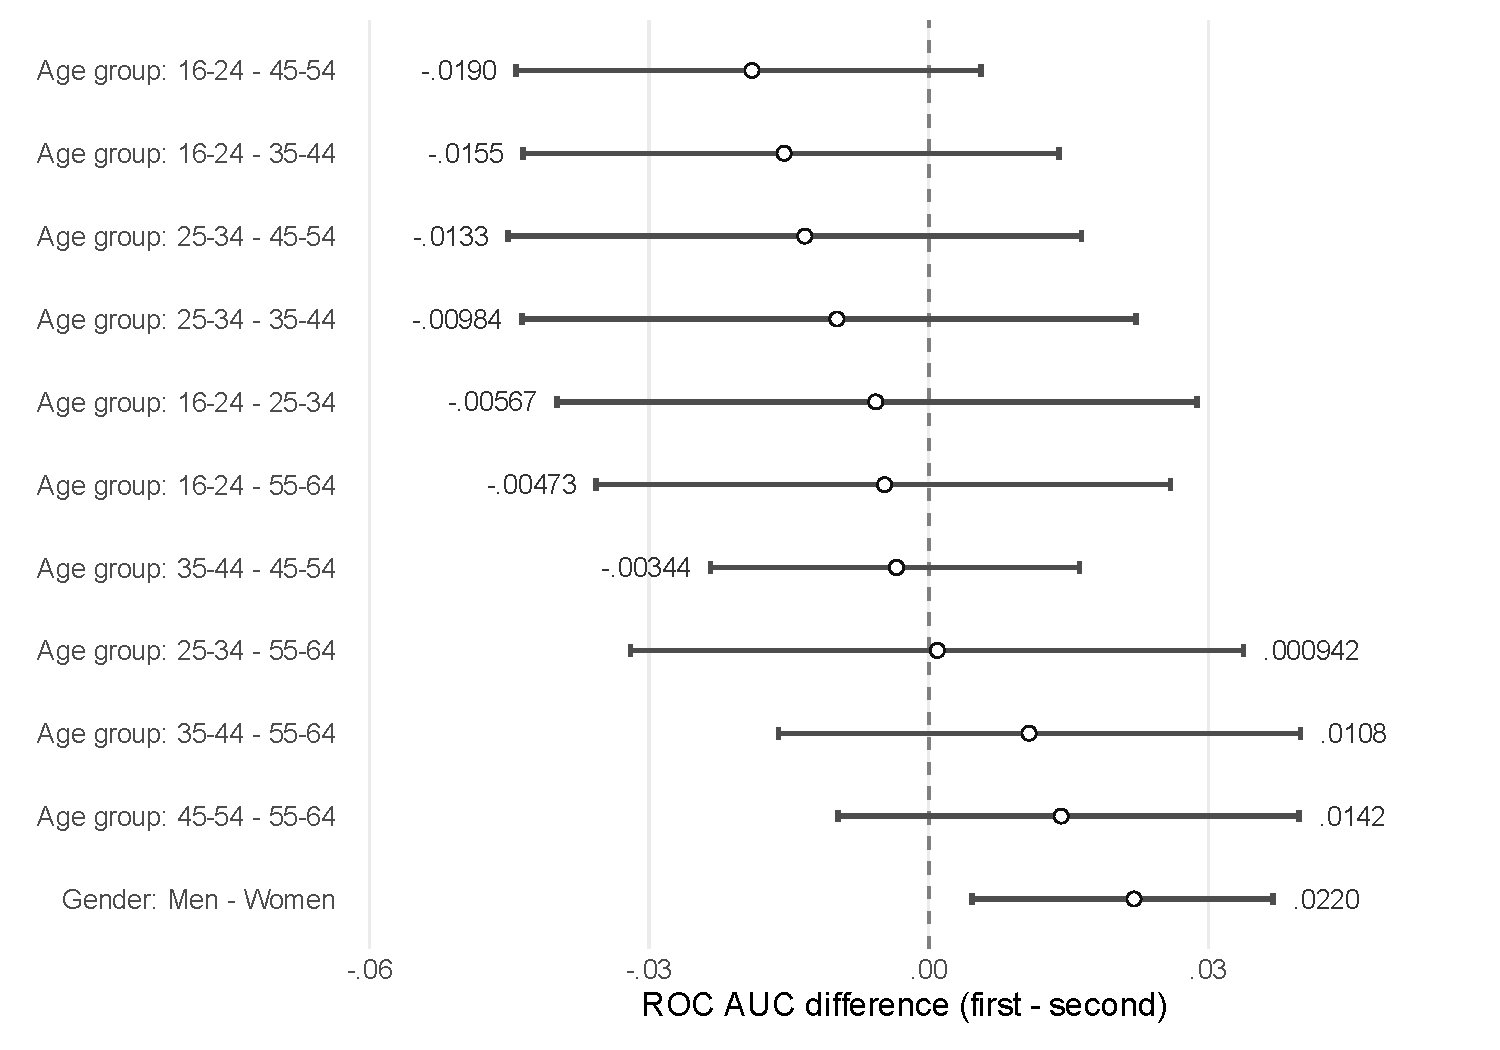
\includegraphics[width=.98\linewidth,height=5.6in,keepaspectratio]{shild/figures/shild_g7_subgroup_contrasts.pdf}
\par\smallskip{\raggedright\small\textit{Note.} Points are first-minus-second differences; interval whiskers are unadjusted conditional 95\% bootstrap intervals. Model-training variation is excluded, and no significance claim is made.\par}
\end{figure}
\clearpage
\begin{figure}[p]
\caption{SHILD: ALE for Age}
\label{supp:shild_rich_ale_1d__age}
\centering
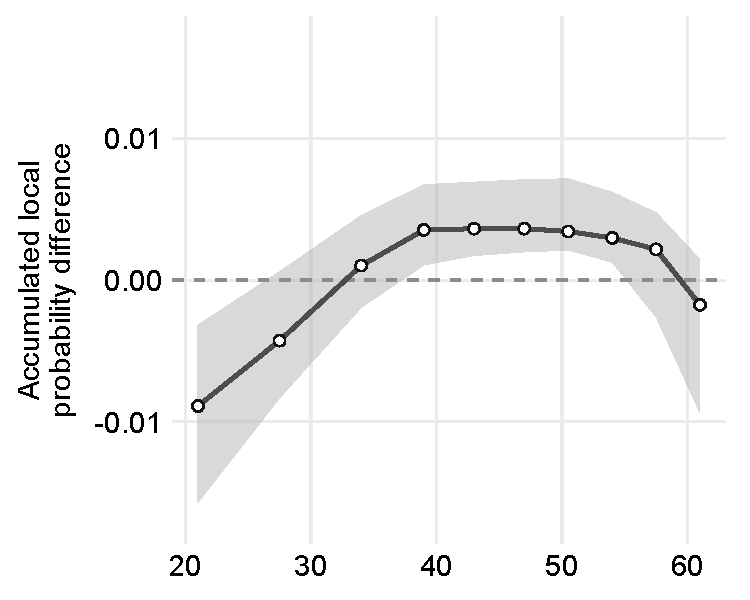
\includegraphics[width=.98\linewidth,height=5.6in,keepaspectratio]{shild/figures/shild_rich_ale_1d__age.pdf}
\par\smallskip{\raggedright\small\textit{Note.} Horizontal axis: Age, measured in years. Ribbon: pointwise 95\% respondent-bootstrap percentile interval from complete learner refits; not a simultaneous band and conditional on the fixed learner specification. The curve is centered accumulated local prediction differences from the XGBoost fit to the full analytic sample over supported empirical intervals. Cells below 20 reference observations are suppressed. Bands use 500 complete fixed-pipeline refits on common boundaries; they omit model-selection variation.\par}
\end{figure}
\clearpage
\begin{figure}[p]
\caption{SHILD: ALE for Height (E1)}
\label{supp:shild_rich_ale_1d__e1}
\centering
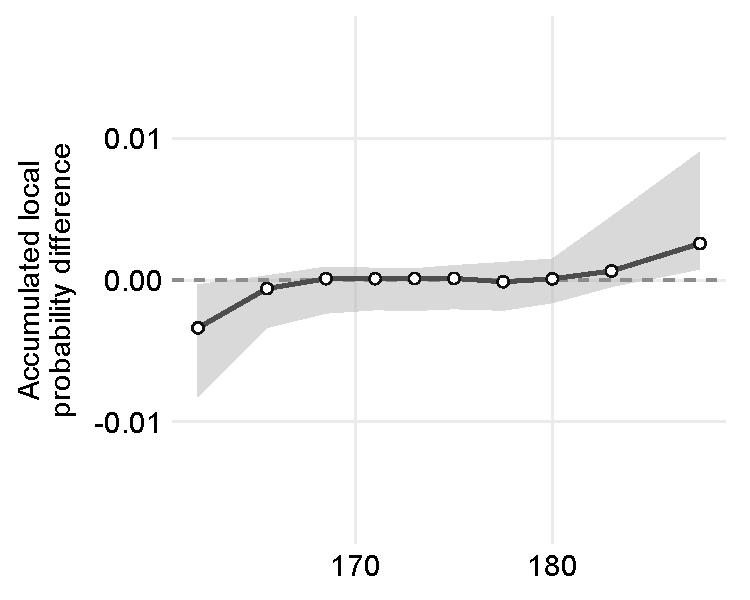
\includegraphics[width=.98\linewidth,height=5.6in,keepaspectratio]{shild/figures/shild_rich_ale_1d__e1.pdf}
\par\smallskip{\raggedright\small\textit{Note.} Horizontal axis: Height (E1), measured in centimeters. Ribbon: pointwise 95\% respondent-bootstrap percentile interval from complete learner refits; not a simultaneous band and conditional on the fixed learner specification. The curve is centered accumulated local prediction differences from the XGBoost fit to the full analytic sample over supported empirical intervals. Cells below 20 reference observations are suppressed. Bands use 500 complete fixed-pipeline refits on common boundaries; they omit model-selection variation.\par}
\end{figure}
\clearpage
\begin{figure}[p]
\caption{SHILD: ALE for Spending on medicine and nutritional supplements in the past year (M6)}
\label{supp:shild_rich_ale_1d__m6}
\centering
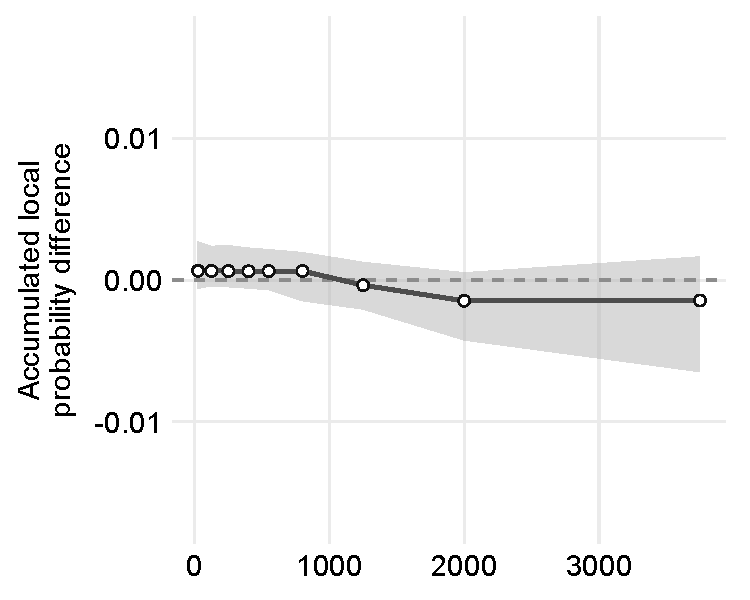
\includegraphics[width=.98\linewidth,height=5.6in,keepaspectratio]{shild/figures/shild_rich_ale_1d__m6.pdf}
\par\smallskip{\raggedright\small\textit{Note.} Horizontal axis: Spending on medicine and nutritional supplements in the past year (M6), measured in Danish kroner. Ribbon: pointwise 95\% respondent-bootstrap percentile interval from complete learner refits; not a simultaneous band and conditional on the fixed learner specification. The curve is centered accumulated local prediction differences from the XGBoost fit to the full analytic sample over supported empirical intervals. Cells below 20 reference observations are suppressed. Bands use 500 complete fixed-pipeline refits on common boundaries; they omit model-selection variation.\par}
\end{figure}
\clearpage
\begin{figure}[p]
\caption{SHILD: ALE for Weight (E2)}
\label{supp:shild_rich_ale_1d__e2}
\centering
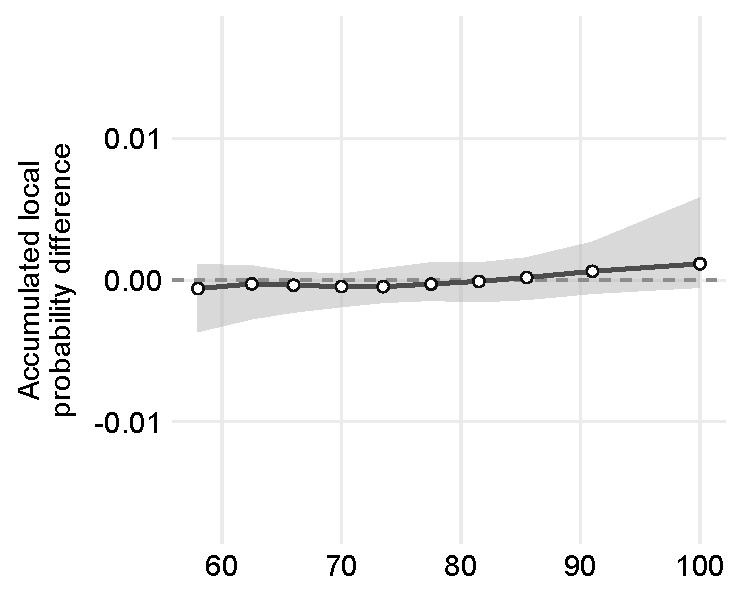
\includegraphics[width=.98\linewidth,height=5.6in,keepaspectratio]{shild/figures/shild_rich_ale_1d__e2.pdf}
\par\smallskip{\raggedright\small\textit{Note.} Horizontal axis: Weight (E2), measured in kilograms. Ribbon: pointwise 95\% respondent-bootstrap percentile interval from complete learner refits; not a simultaneous band and conditional on the fixed learner specification. The curve is centered accumulated local prediction differences from the XGBoost fit to the full analytic sample over supported empirical intervals. Cells below 20 reference observations are suppressed. Bands use 500 complete fixed-pipeline refits on common boundaries; they omit model-selection variation.\par}
\end{figure}
\clearpage
\begin{figure}[p]
\caption{SHILD: aggregate ICE for Age}
\label{supp:shild_rich_ice_quantiles__age}
\centering
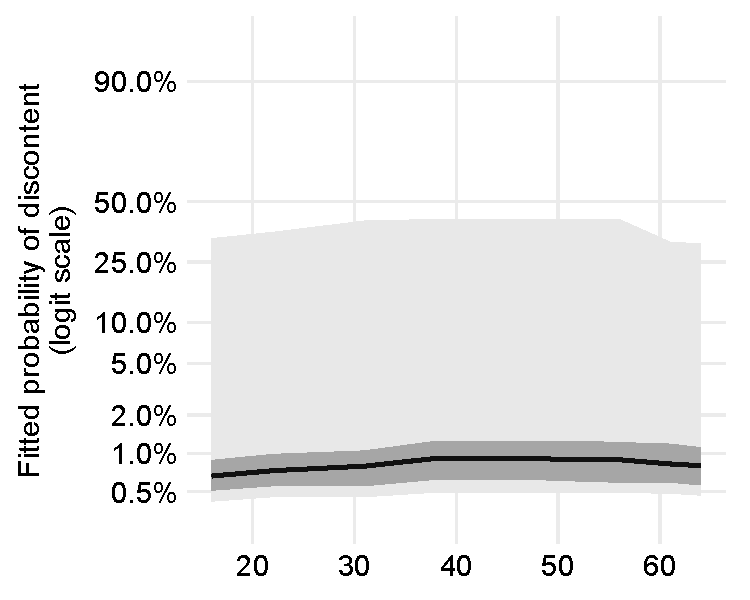
\includegraphics[width=.98\linewidth,height=5.6in,keepaspectratio]{shild/figures/shild_rich_ice_quantiles__age.pdf}
\par\smallskip

\includegraphics[width=.98\linewidth]{shild/figures/shild_rich_ice_quantiles__legend.pdf}
\par\smallskip{\raggedright\small\textit{Note.} Horizontal axis: Age, measured in years. The outer band is pointwise q05-q95, the inner band is q25-q75, and the line is the pointwise median across row-level ICE curves; these are descriptive curve quantiles, not confidence intervals. Quantiles summarize the 30 reference-case prediction curves at each queried value. Queries may leave empirical support and are not causal effects or feasible changes for individuals.\par}
\end{figure}
\clearpage
\begin{figure}[p]
\caption{SHILD: aggregate ICE for Height (E1)}
\label{supp:shild_rich_ice_quantiles__e1}
\centering
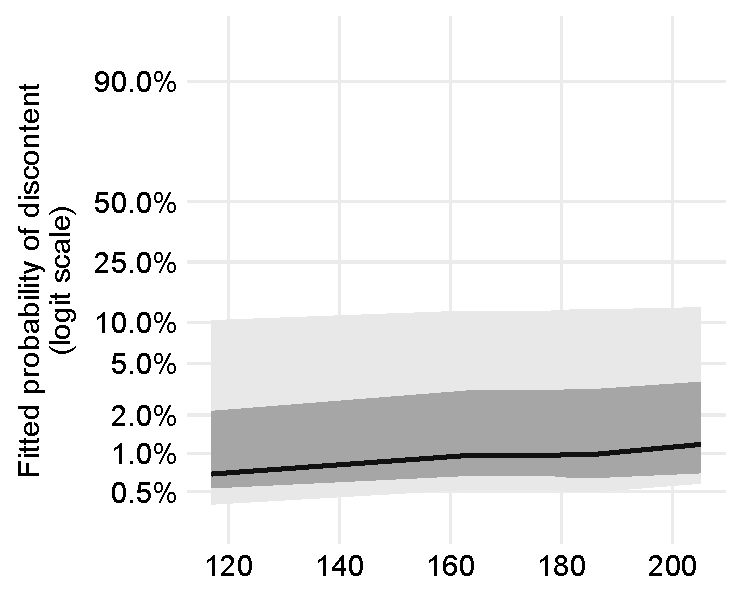
\includegraphics[width=.98\linewidth,height=5.6in,keepaspectratio]{shild/figures/shild_rich_ice_quantiles__e1.pdf}
\par\smallskip{\raggedright\small\textit{Note.} Horizontal axis: Height (E1), measured in centimeters. The outer band is pointwise q05-q95, the inner band is q25-q75, and the line is the pointwise median across row-level ICE curves; these are descriptive curve quantiles, not confidence intervals. Quantiles summarize the 30 reference-case prediction curves at each queried value. Queries may leave empirical support and are not causal effects or feasible changes for individuals.\par}
\end{figure}
\clearpage
\begin{figure}[p]
\caption{SHILD: aggregate ICE for Spending on medicine and nutritional supplements in the past year (M6)}
\label{supp:shild_rich_ice_quantiles__m6}
\centering
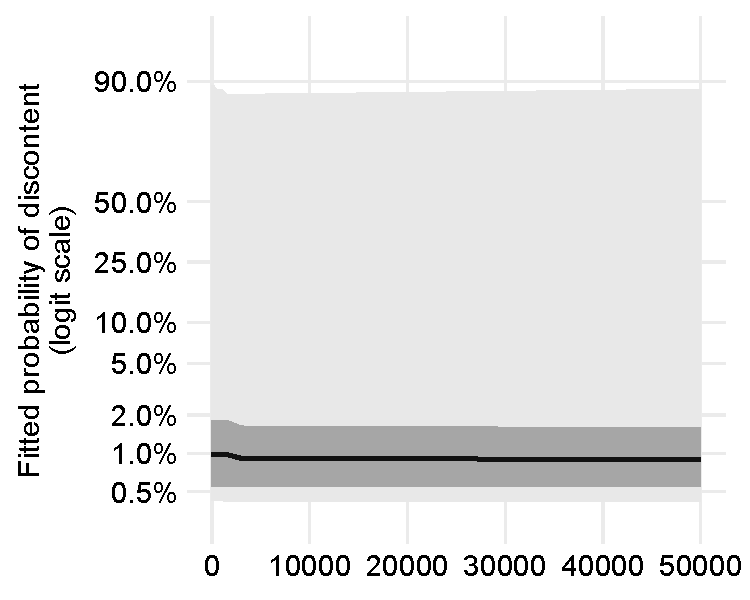
\includegraphics[width=.98\linewidth,height=5.6in,keepaspectratio]{shild/figures/shild_rich_ice_quantiles__m6.pdf}
\par\smallskip{\raggedright\small\textit{Note.} Horizontal axis: Spending on medicine and nutritional supplements in the past year (M6), measured in Danish kroner. The outer band is pointwise q05-q95, the inner band is q25-q75, and the line is the pointwise median across row-level ICE curves; these are descriptive curve quantiles, not confidence intervals. Quantiles summarize the 30 reference-case prediction curves at each queried value. Queries may leave empirical support and are not causal effects or feasible changes for individuals.\par}
\end{figure}
\clearpage
\begin{figure}[p]
\caption{SHILD: aggregate ICE for Weight (E2)}
\label{supp:shild_rich_ice_quantiles__e2}
\centering
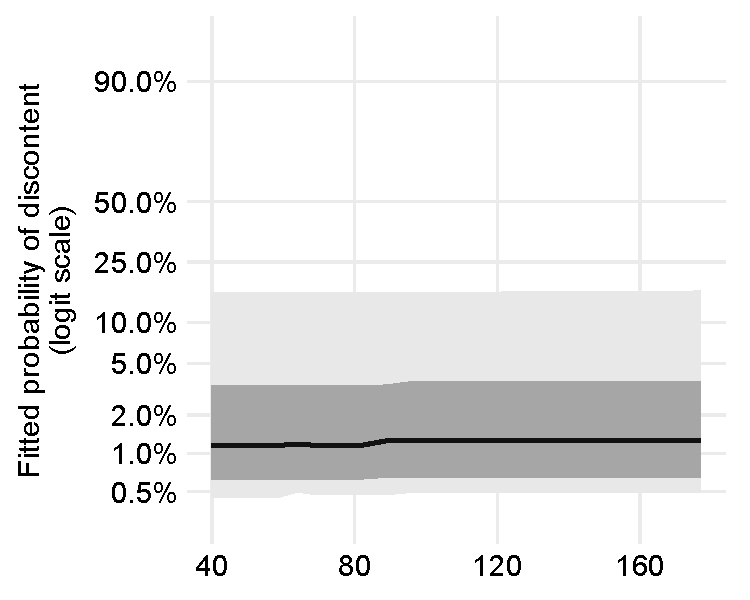
\includegraphics[width=.98\linewidth,height=5.6in,keepaspectratio]{shild/figures/shild_rich_ice_quantiles__e2.pdf}
\par\smallskip{\raggedright\small\textit{Note.} Horizontal axis: Weight (E2), measured in kilograms. The outer band is pointwise q05-q95, the inner band is q25-q75, and the line is the pointwise median across row-level ICE curves; these are descriptive curve quantiles, not confidence intervals. Quantiles summarize the 30 reference-case prediction curves at each queried value. Queries may leave empirical support and are not causal effects or feasible changes for individuals.\par}
\end{figure}
\clearpage
\begin{figure}[p]
\caption{SHILD second-order ALE interaction surface}
\label{supp:shild_rich_ale_2d}
\centering
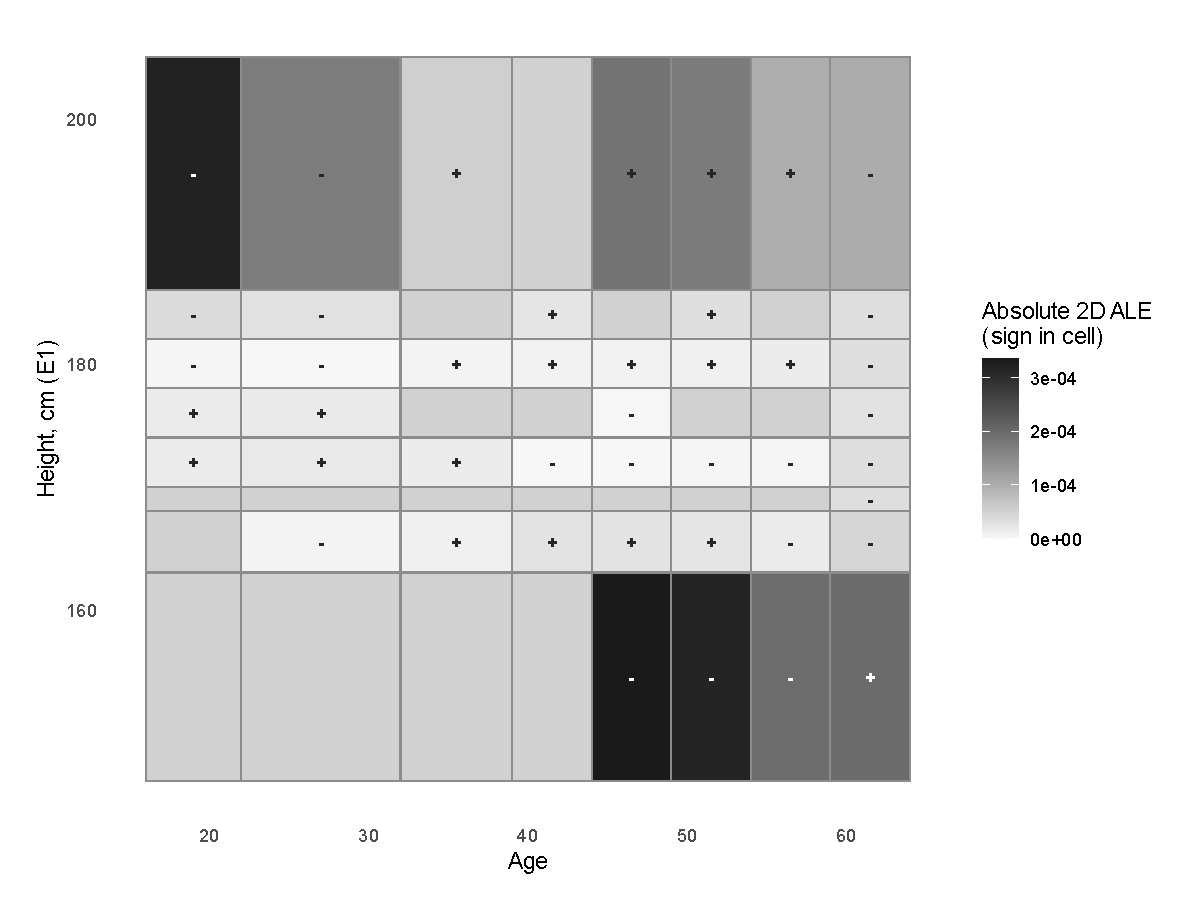
\includegraphics[width=.98\linewidth,height=5.6in,keepaspectratio]{shild/figures/shild_rich_ale_2d.pdf}
\par\smallskip{\raggedright\small\textit{Note.} First-order effects are removed; irregular rectangles follow empirical cells, and gray cells have n < 20. Model-fitting uncertainty is not represented. Age is measured in years and height in centimeters.\par}
\end{figure}
\clearpage
\begin{figure}[p]
\caption{SHILD raw-probability dispersion across similarly accurate learners}
\label{supp:shild_prediction_multiplicity}
\centering
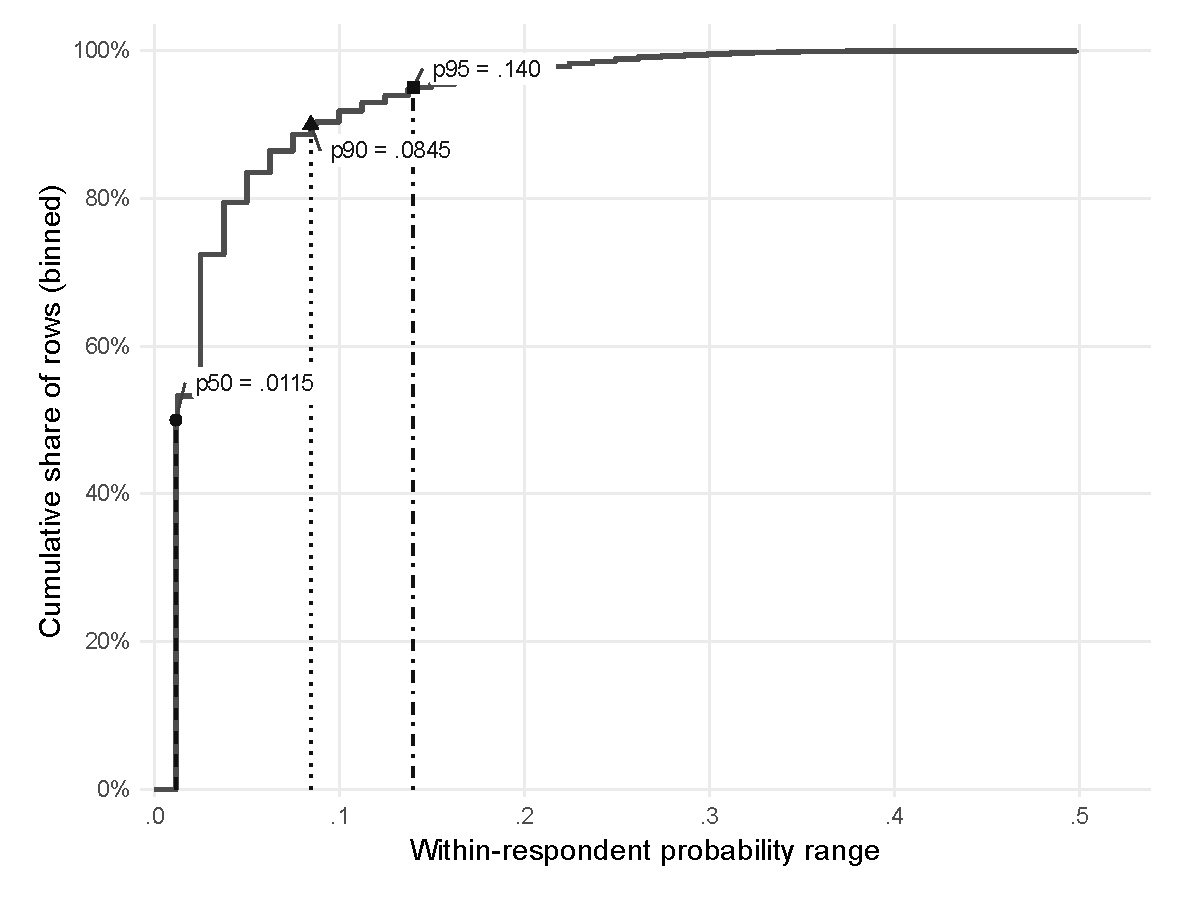
\includegraphics[width=.98\linewidth,height=5.6in,keepaspectratio]{shild/figures/shild_prediction_multiplicity.pdf}
\par\smallskip{\raggedright\small\textit{Note.} Stepwise cumulative held-out summary from shareable fixed-width bin counts, with exact aggregate median, 90th, and 95th percentile anchors. The steps do not imply continuous or row-level resolution; labeled ranges are not confidence intervals. Range means the largest minus the smallest held-out prediction of the similarly accurate learners for the same respondent or student. The cumulative step curve summarizes fixed-width bins; separately labeled quantile anchors retain exact aggregate values.\par}
\end{figure}
\clearpage
\begin{figure}[p]
\caption{PISA, first plausible value: flexible held-out calibration illustration}
\label{supp:pisa_g3_calibration}
\centering
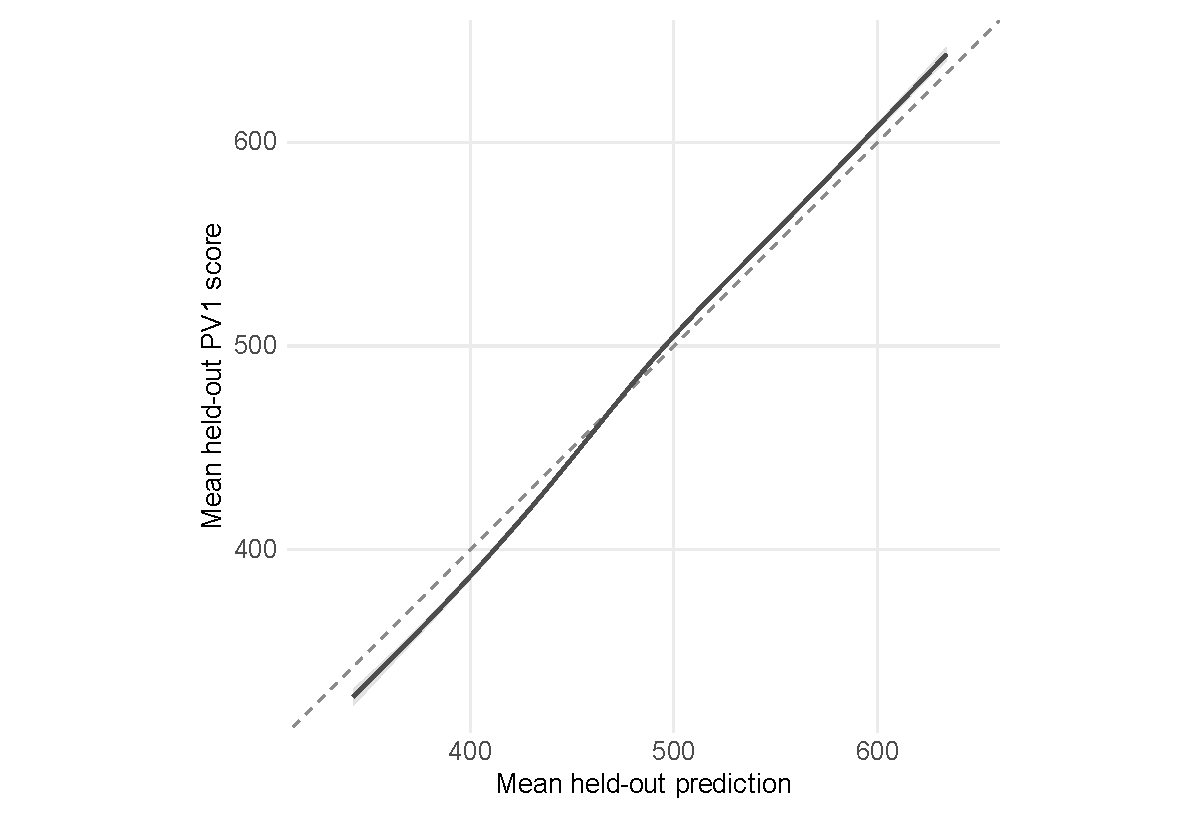
\includegraphics[width=.98\linewidth,height=5.6in,keepaspectratio]{pisa/figures/pisa_g3_calibration.pdf}
\par\smallskip{\raggedright\small\textit{Note.} The curve is a natural cubic regression spline with four degrees of freedom; the band is a pointwise 95\% school-within-country bootstrap percentile interval conditional on the supplied held-out predictions. The band is not simultaneous and omits model-training and plausible-value uncertainty; all ten plausible-value summaries are reported in the accompanying tables.\par}
\end{figure}
\clearpage
\begin{figure}[p]
\caption{PISA, first plausible value: technical subgroup boundary diagnostic, by gender}
\label{supp:pisa_g7_subgroups__audit_gender}
\centering
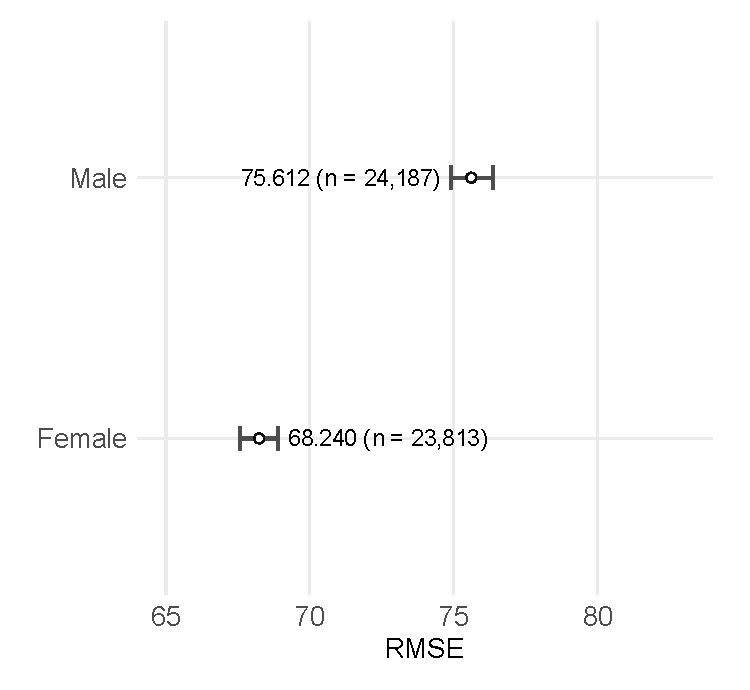
\includegraphics[width=.98\linewidth,height=5.6in,keepaspectratio]{pisa/figures/pisa_g7_subgroups__audit_gender.pdf}
\par\smallskip{\raggedright\small\textit{Note.} School-clustered 95\% percentile-bootstrap intervals are stratified within country and conditional on held-out predictions. The common RMSE axis spans 64–84 points; this is not a population subgroup claim.\par}
\end{figure}
\clearpage
\begin{figure}[p]
\caption{PISA, first plausible value: technical subgroup boundary diagnostic, by immigration background}
\label{supp:pisa_g7_subgroups__audit_immigration}
\centering
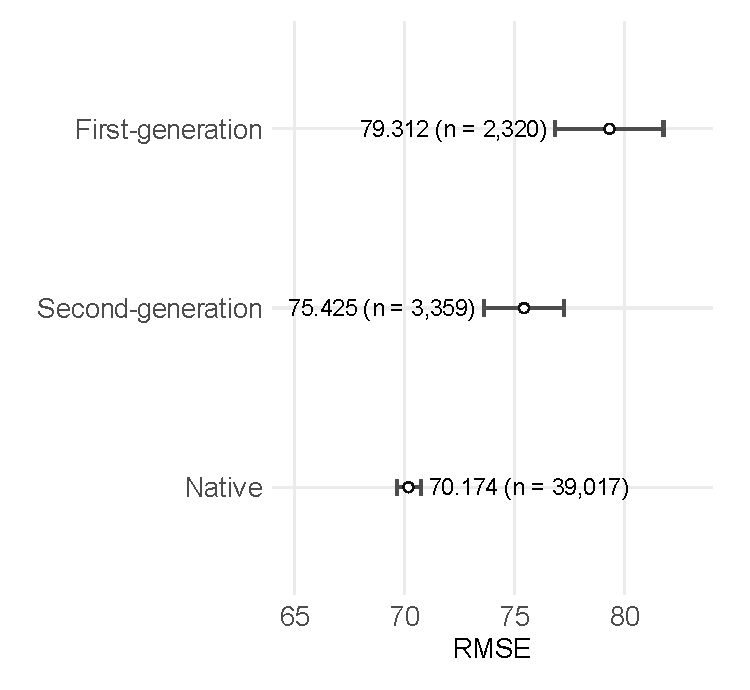
\includegraphics[width=.98\linewidth,height=5.6in,keepaspectratio]{pisa/figures/pisa_g7_subgroups__audit_immigration.pdf}
\par\smallskip{\raggedright\small\textit{Note.} School-clustered 95\% percentile-bootstrap intervals are stratified within country and conditional on held-out predictions. The common RMSE axis spans 64–84 points; this is not a population subgroup claim.\par}
\end{figure}
\clearpage
\begin{figure}[p]
\caption{PISA, first plausible value: technical subgroup RMSE contrasts}
\label{supp:pisa_g7_subgroup_contrasts}
\centering
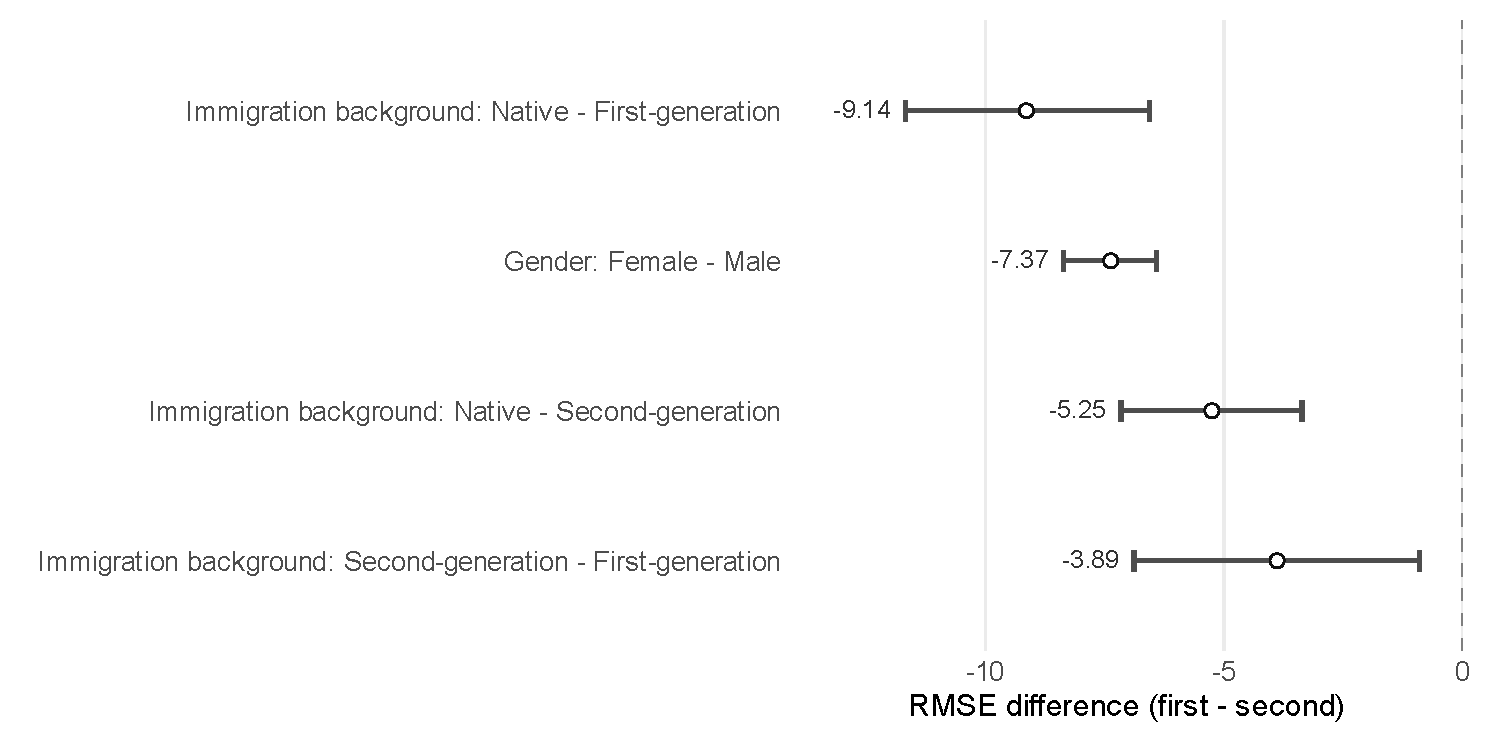
\includegraphics[width=.98\linewidth,height=5.6in,keepaspectratio]{pisa/figures/pisa_g7_subgroup_contrasts.pdf}
\par\smallskip{\raggedright\small\textit{Note.} Points are first-minus-second RMSE differences; whiskers are school-clustered 95\% percentile-bootstrap intervals stratified within country and conditional on held-out predictions. This is a technical boundary diagnostic, not a population subgroup claim.\par}
\end{figure}
\clearpage
\begin{figure}[p]
\caption{PISA: ALE for Hypothetical test effort (EFFORT2)}
\label{supp:pisa_rich_ale_1d__effort2}
\centering
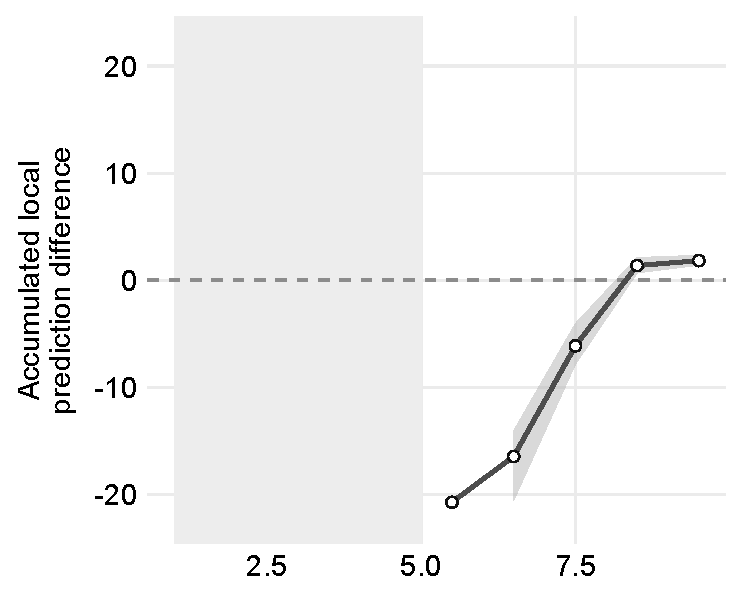
\includegraphics[width=.98\linewidth,height=5.6in,keepaspectratio]{pisa/figures/pisa_rich_ale_1d__effort2.pdf}
\par\smallskip{\raggedright\small\textit{Note.} Horizontal axis: Hypothetical test effort (EFFORT2), measured in reported effort-rating points, not actual effort (EFFORT1). Ribbon: pointwise 95\% country-stratified school-bootstrap percentile interval from complete learner refits; not simultaneous and conditional on the first plausible value and the fixed learner specification. A ribbon is omitted where fewer than 80\% of refits meet the interval-support threshold. The curve is centered accumulated local prediction differences from the XGBoost fit to the full analytic sample over supported empirical intervals. Cells below 20 reference observations are suppressed. Bands use 500 complete fixed-pipeline refits on common boundaries; they omit model-selection variation.\par}
\end{figure}
\clearpage
\begin{figure}[p]
\caption{PISA: ALE for Highest parental education (PARED)}
\label{supp:pisa_rich_ale_1d__pared}
\centering
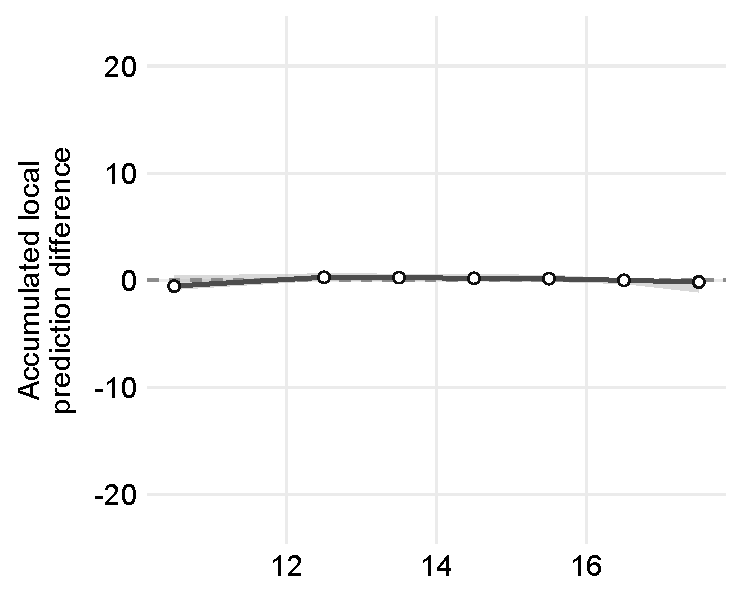
\includegraphics[width=.98\linewidth,height=5.6in,keepaspectratio]{pisa/figures/pisa_rich_ale_1d__pared.pdf}
\par\smallskip{\raggedright\small\textit{Note.} Horizontal axis: Highest parental education (PARED), measured in years of schooling. Ribbon: pointwise 95\% country-stratified school-bootstrap percentile interval from complete learner refits; not simultaneous and conditional on the first plausible value and the fixed learner specification. A ribbon is omitted where fewer than 80\% of refits meet the interval-support threshold. The curve is centered accumulated local prediction differences from the XGBoost fit to the full analytic sample over supported empirical intervals. Cells below 20 reference observations are suppressed. Bands use 500 complete fixed-pipeline refits on common boundaries; they omit model-selection variation.\par}
\end{figure}
\clearpage
\begin{figure}[p]
\caption{PISA: ALE for Highest parental occupational status (HISEI)}
\label{supp:pisa_rich_ale_1d__hisei}
\centering
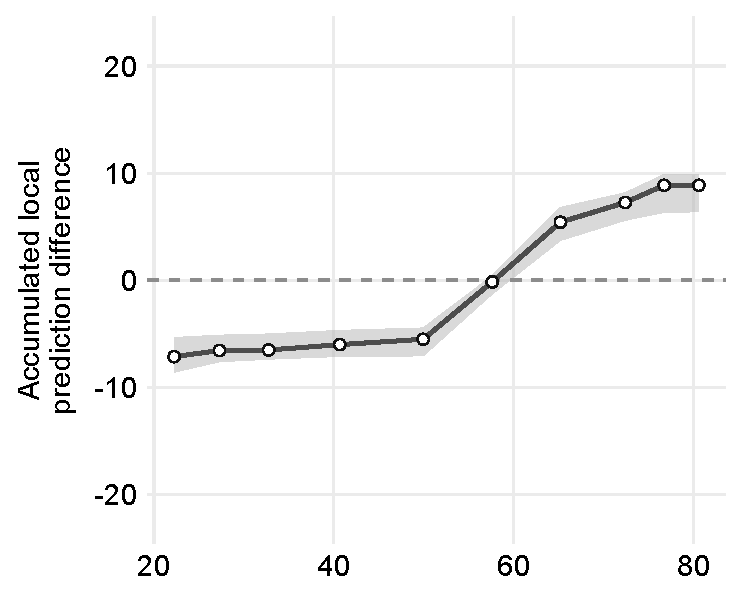
\includegraphics[width=.98\linewidth,height=5.6in,keepaspectratio]{pisa/figures/pisa_rich_ale_1d__hisei.pdf}
\par\smallskip{\raggedright\small\textit{Note.} Horizontal axis: Highest parental occupational status (HISEI), measured in occupational-status index points. Ribbon: pointwise 95\% country-stratified school-bootstrap percentile interval from complete learner refits; not simultaneous and conditional on the first plausible value and the fixed learner specification. A ribbon is omitted where fewer than 80\% of refits meet the interval-support threshold. The curve is centered accumulated local prediction differences from the XGBoost fit to the full analytic sample over supported empirical intervals. Cells below 20 reference observations are suppressed. Bands use 500 complete fixed-pipeline refits on common boundaries; they omit model-selection variation.\par}
\end{figure}
\clearpage
\begin{figure}[p]
\caption{PISA: ALE for Enjoyment of reading (JOYREAD)}
\label{supp:pisa_rich_ale_1d__joyread}
\centering
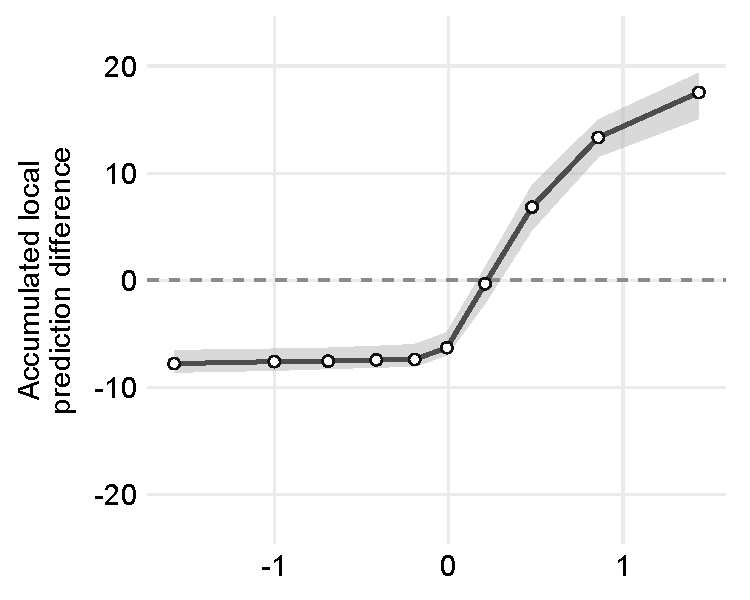
\includegraphics[width=.98\linewidth,height=5.6in,keepaspectratio]{pisa/figures/pisa_rich_ale_1d__joyread.pdf}
\par\smallskip{\raggedright\small\textit{Note.} Horizontal axis: Enjoyment of reading (JOYREAD), measured in standardized weighted-likelihood index units. Ribbon: pointwise 95\% country-stratified school-bootstrap percentile interval from complete learner refits; not simultaneous and conditional on the first plausible value and the fixed learner specification. A ribbon is omitted where fewer than 80\% of refits meet the interval-support threshold. The curve is centered accumulated local prediction differences from the XGBoost fit to the full analytic sample over supported empirical intervals. Cells below 20 reference observations are suppressed. Bands use 500 complete fixed-pipeline refits on common boundaries; they omit model-selection variation.\par}
\end{figure}
\clearpage
\begin{figure}[p]
\caption{PISA: aggregate ICE for Hypothetical test effort (EFFORT2)}
\label{supp:pisa_rich_ice_quantiles__effort2}
\centering
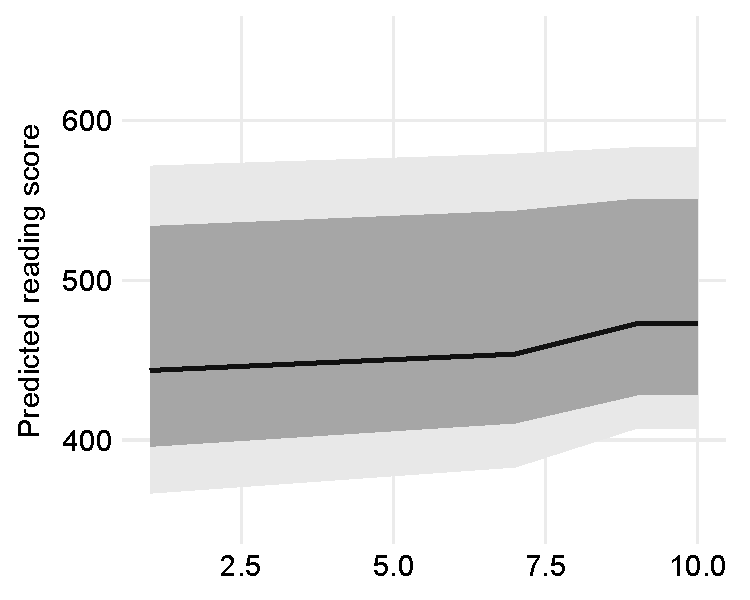
\includegraphics[width=.98\linewidth,height=5.6in,keepaspectratio]{pisa/figures/pisa_rich_ice_quantiles__effort2.pdf}
\par\smallskip

\includegraphics[width=.98\linewidth]{pisa/figures/pisa_rich_ice_quantiles__legend.pdf}
\par\smallskip{\raggedright\small\textit{Note.} Horizontal axis: Hypothetical test effort (EFFORT2), measured in reported effort-rating points, not actual effort (EFFORT1). The outer light-gray band is pointwise q05-q95, the inner dark-gray band is q25-q75, and the line is the pointwise median. All panels use the same labeled 350-650 reading-score scale; these are curve quantiles, not confidence intervals. Quantiles summarize the 30 reference-case prediction curves at each queried value. Queries may leave empirical support and are not causal effects or feasible changes for individuals.\par}
\end{figure}
\clearpage
\begin{figure}[p]
\caption{PISA: aggregate ICE for Highest parental education (PARED)}
\label{supp:pisa_rich_ice_quantiles__pared}
\centering
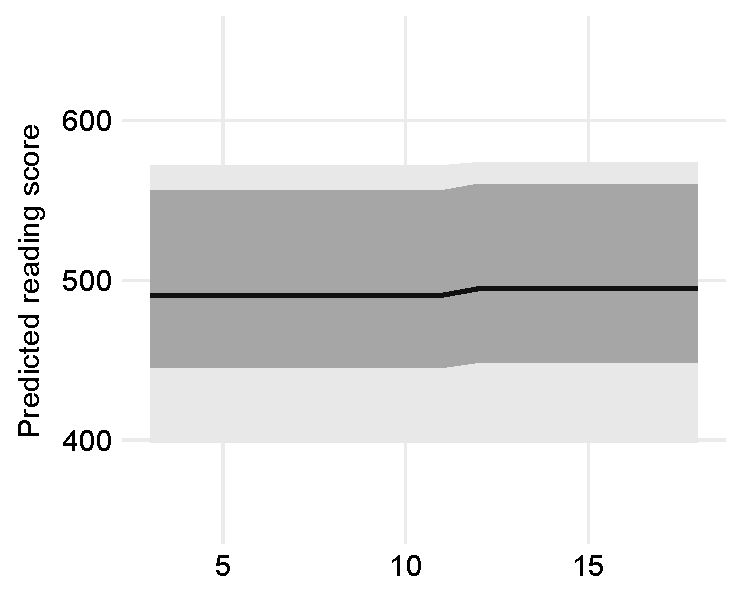
\includegraphics[width=.98\linewidth,height=5.6in,keepaspectratio]{pisa/figures/pisa_rich_ice_quantiles__pared.pdf}
\par\smallskip{\raggedright\small\textit{Note.} Horizontal axis: Highest parental education (PARED), measured in years of schooling. The outer light-gray band is pointwise q05-q95, the inner dark-gray band is q25-q75, and the line is the pointwise median. All panels use the same labeled 350-650 reading-score scale; these are curve quantiles, not confidence intervals. Quantiles summarize the 30 reference-case prediction curves at each queried value. Queries may leave empirical support and are not causal effects or feasible changes for individuals.\par}
\end{figure}
\clearpage
\begin{figure}[p]
\caption{PISA: aggregate ICE for Highest parental occupational status (HISEI)}
\label{supp:pisa_rich_ice_quantiles__hisei}
\centering
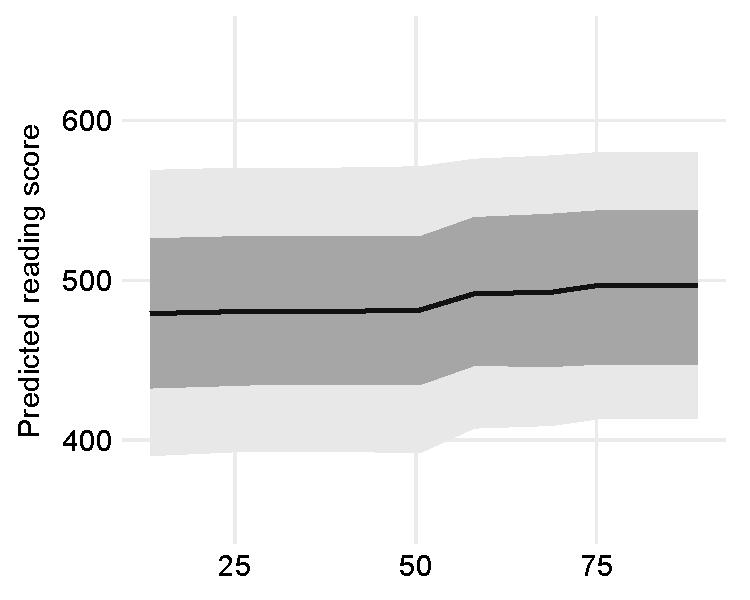
\includegraphics[width=.98\linewidth,height=5.6in,keepaspectratio]{pisa/figures/pisa_rich_ice_quantiles__hisei.pdf}
\par\smallskip{\raggedright\small\textit{Note.} Horizontal axis: Highest parental occupational status (HISEI), measured in occupational-status index points. The outer light-gray band is pointwise q05-q95, the inner dark-gray band is q25-q75, and the line is the pointwise median. All panels use the same labeled 350-650 reading-score scale; these are curve quantiles, not confidence intervals. Quantiles summarize the 30 reference-case prediction curves at each queried value. Queries may leave empirical support and are not causal effects or feasible changes for individuals.\par}
\end{figure}
\clearpage
\begin{figure}[p]
\caption{PISA: aggregate ICE for Enjoyment of reading (JOYREAD)}
\label{supp:pisa_rich_ice_quantiles__joyread}
\centering
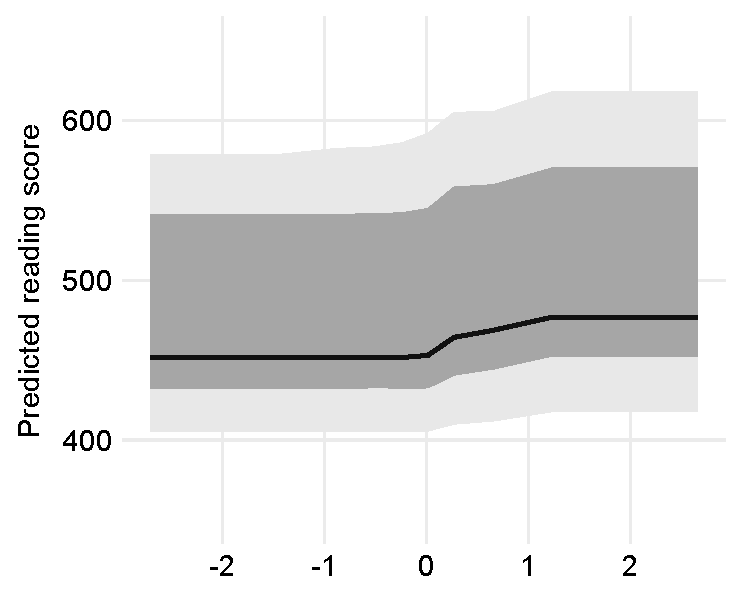
\includegraphics[width=.98\linewidth,height=5.6in,keepaspectratio]{pisa/figures/pisa_rich_ice_quantiles__joyread.pdf}
\par\smallskip{\raggedright\small\textit{Note.} Horizontal axis: Enjoyment of reading (JOYREAD), measured in standardized weighted-likelihood index units. The outer light-gray band is pointwise q05-q95, the inner dark-gray band is q25-q75, and the line is the pointwise median. All panels use the same labeled 350-650 reading-score scale; these are curve quantiles, not confidence intervals. Quantiles summarize the 30 reference-case prediction curves at each queried value. Queries may leave empirical support and are not causal effects or feasible changes for individuals.\par}
\end{figure}
\clearpage
\begin{figure}[p]
\caption{PISA, first plausible value: accumulated local interaction surface}
\label{supp:pisa_rich_ale_2d}
\centering
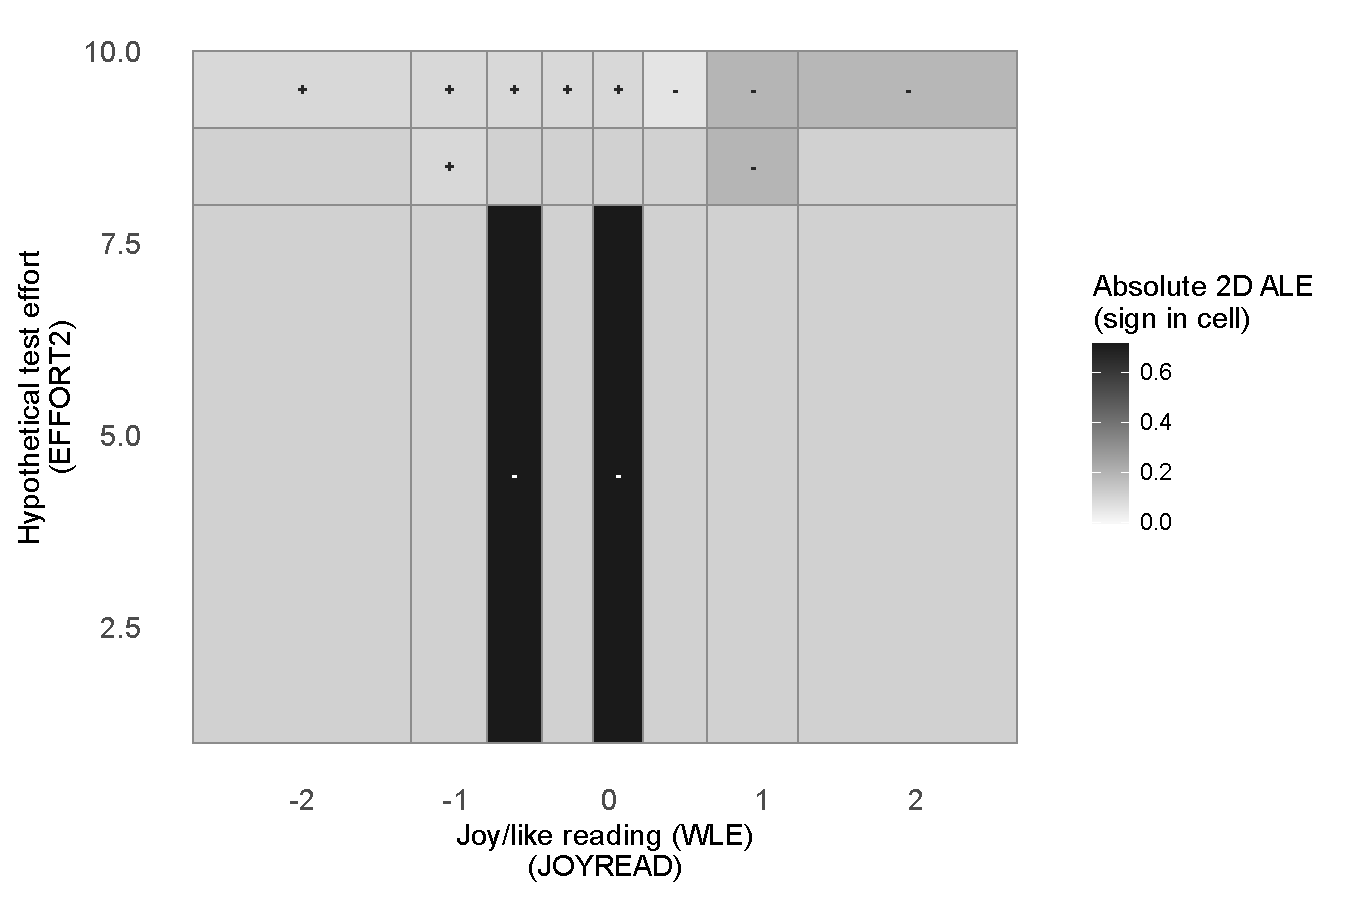
\includegraphics[width=.98\linewidth,height=5.6in,keepaspectratio]{pisa/figures/pisa_rich_ale_2d.pdf}
\par\smallskip{\raggedright\small\textit{Note.} Irregular rectangles follow empirical cell boundaries; gray cells have fewer than 20 sampled observations. Model-fitting uncertainty is not represented. The variables are the standardized JOYREAD index and hypothetical test effort EFFORT2 (rating points), not actual effort EFFORT1. First-order effects are removed.\par}
\end{figure}
\clearpage
\begin{figure}[p]
\caption{PISA, first plausible value: differences in individual predictions across similarly accurate learners}
\label{supp:pisa_prediction_multiplicity}
\centering
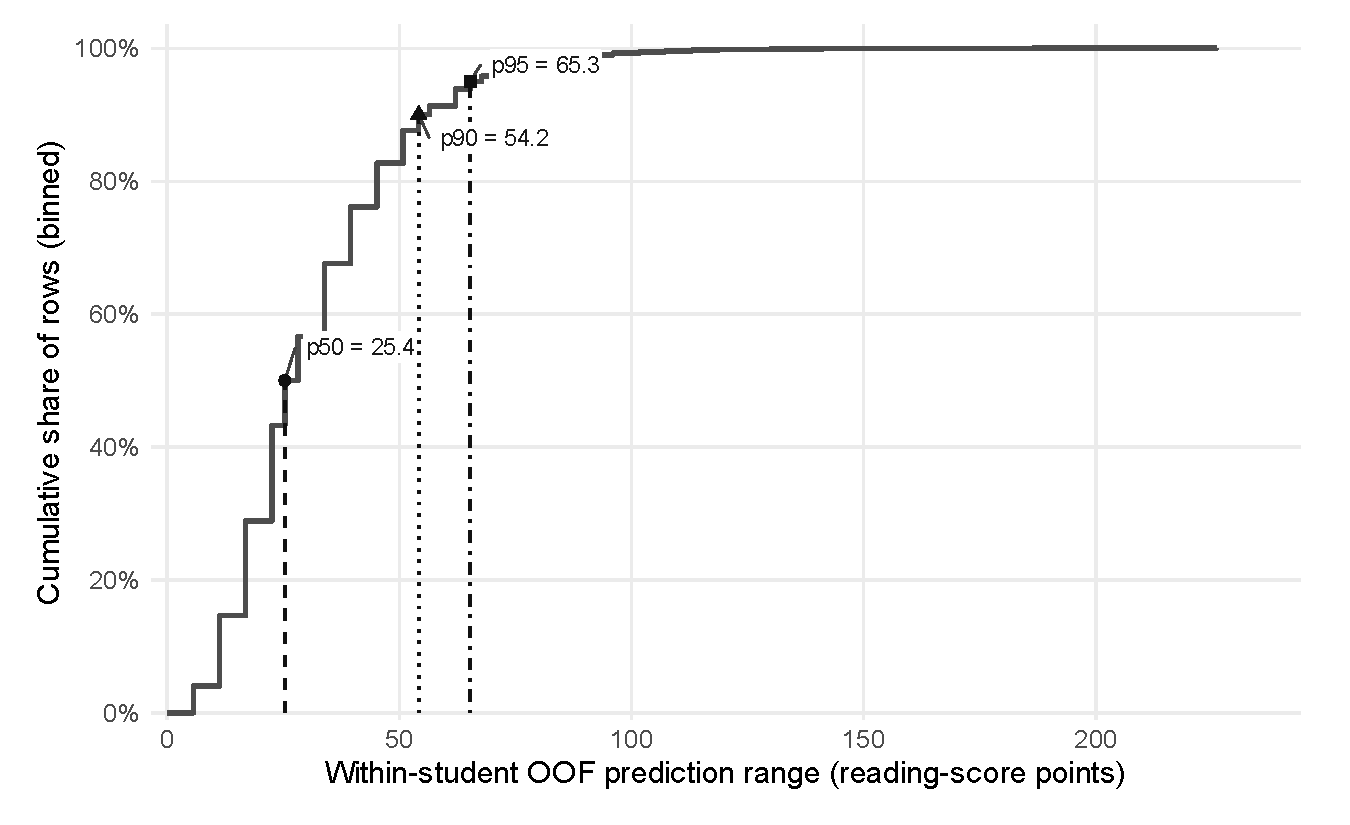
\includegraphics[width=.98\linewidth,height=5.6in,keepaspectratio]{pisa/figures/pisa_prediction_multiplicity.pdf}
\par\smallskip{\raggedright\small\textit{Note.} Stepwise cumulative held-out summary from shareable fixed-width bin counts, with exact aggregate median, 90th, and 95th percentile anchors. The steps do not imply continuous or row-level resolution; row-level ranges remain private. Range means the largest minus the smallest held-out prediction of the similarly accurate learners for the same respondent or student. The cumulative step curve summarizes fixed-width bins; separately labeled quantile anchors retain exact aggregate values.\par}
\end{figure}
\clearpage
\end{document}
